% !TeX program = lualatex
% !TeX encoding = utf8
% !TeX spellcheck = uk_UA
% !BIB program = bibtex8

% !!!!!!!!!!!!!!!!!!!!!!!!!!!!!!!!!!!!!!!!!!!!!!!!!!!!!!!!!!!!!!!!!!!!!!!!!!!!!! %
% !!!!!!!!!!!!!!!! Add path to pygmentize.exe to the system path !!!!!!!!!!!!!!! %
% !!!!!!!!!!!!!!!!!!!!!!!!!!!!!!!!!!!!!!!!!!!!!!!!!!!!!!!!!!!!!!!!!!!!!!!!!!!!!! %

\documentclass[14pt]{extarticle}
	\usepackage{polyglossia}
	\setmainlanguage{ukrainian}
	\setotherlanguages{english, russian}
	\setsansfont{CMU Sans Serif}
	\setmainfont[Ligatures=TeX]{CMU Serif}
	\setmonofont{Consolas}
	\usepackage{minted, xcolor, graphicx}
	\definecolor{lightgray}{gray}{0.95}
	\renewcommand\listoflistingscaption{List of source codes}
	\renewcommand\theFancyVerbLine{\scriptsize\arabic{FancyVerbLine}}
	%------------------------------------------------------------------
	\RequirePackage[%
	a4paper,%
	footskip=1cm,%
	headsep=0.3cm,% 
	top=2cm, %поле сверху
	bottom=2cm, %поле снизу
	left=2cm, %поле ліворуч
	right=2cm, %поле праворуч
	]{geometry}
	%-------------Подавление висячих строк--------------------------------
	\clubpenalty =10000
	\widowpenalty=10000
	%-------------Інтервали-----------------------------------------------
	\setlength{\parskip}{0.5ex}%
	\setlength{\parindent}{2.5em}%
	\renewcommand{\baselinestretch}{1.1}
	%---------------------------------------------------------------------
\title{Задача багатьох тіл на прикладі сонячної системи}
\begin{document}
\maketitle

Знайшов в мережі доволі цікаву програму написану на \texttt{Python} яка моделює Сонячну систему. В програмі врахована взаємодія не лише планет із Сонцем, а також взаємодія планет між собою. В систему можна додавати планети, та інші небесні тіла. 

\begin{figure}[h!]
	\centering
	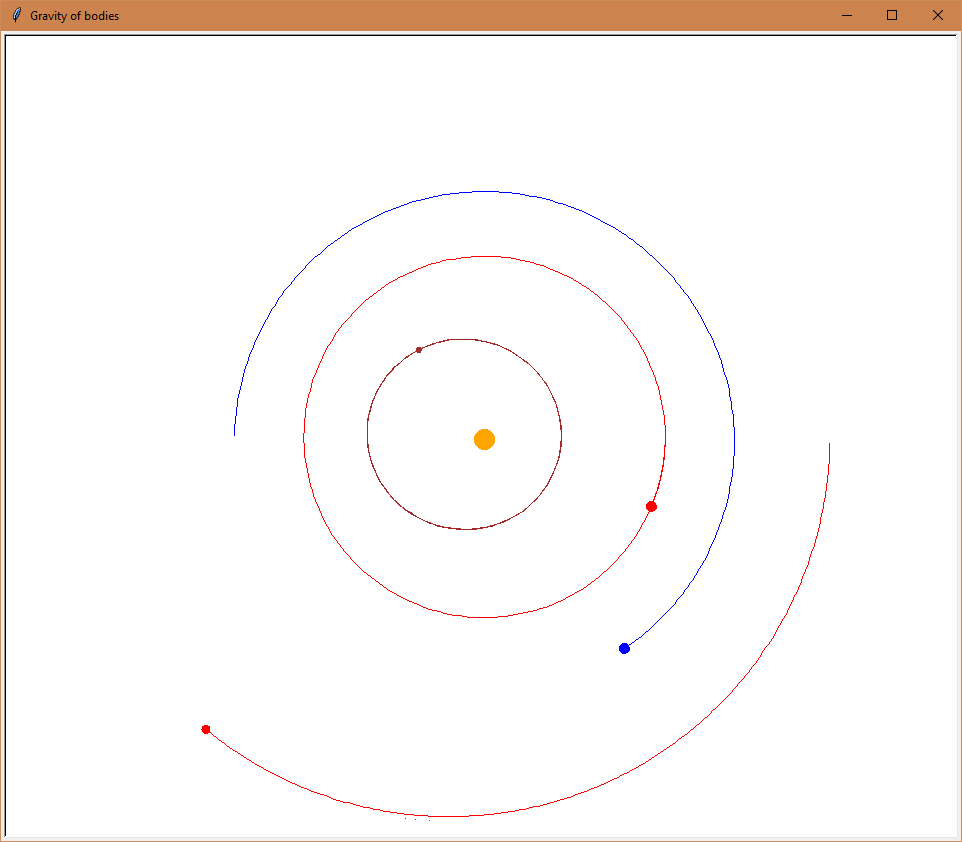
\includegraphics[width=0.7\linewidth]{Pic1}
	\caption{Сонячна система з Сонцем, Меркурієм, Венерою, Землею та Марсом}
	\label{fig:pic1}
\end{figure}



\begin{minted}
[
frame=lines,
framesep=2mm,
baselinestretch=1.2,
bgcolor=lightgray,
fontsize=\footnotesize,
linenos,
breaklines
]
{python}
#!/usr/bin/env python3
#https://fiftyexamples.readthedocs.io/en/latest/gravity.html
import math
from turtle import *

# The gravitational constant G
G = 6.67428e-11
c = 299792458

# Assumed scale: 100 pixels = 1AU.
AU = (149.6e6 * 1000)     # 149.6 million km, in meters.
SCALE = 250 / AU
wn = Screen()
wn.title("Gravity of bodies")      # Set the window title


class Body(Turtle):
    """Subclass of Turtle representing a gravitationally-acting body.

    Extra attributes:
    mass : mass in kg
    vx, vy: x, y velocities in m/s
    px, py: x, y positions in m
    """
    
    name = 'Body'
    mass = None
    vx = vy = 0.0
    px = py = 0.0
    
    def attraction(self, other):
        """(Body): (fx, fy)

        Returns the force exerted upon this body by the other body.
        """
        # Report an error if the other object is the same as this one.
        if self is other:
            raise ValueError("Attraction of object %r to itself requested"
                             % self.name)

        # Compute the distance of the other body.
        sx, sy = self.px, self.py
        ox, oy = other.px, other.py
        dx = (ox-sx)
        dy = (oy-sy)
        d = math.sqrt(dx**2 + dy**2)

        # Report an error if the distance is zero; otherwise we'll
        # get a ZeroDivisionError exception further down.
        if d == 0:
            raise ValueError("Collision between objects %r and %r"
                             % (self.name, other.name))

        # Compute the force of attraction
        f = G * self.mass * other.mass / (d**2) / (math.sqrt(1 - 2*G*other.mass/(d*c**2)))

        # Compute the direction of the force.
        theta = math.atan2(dy, dx)
        fx = math.cos(theta) * f
        fy = math.sin(theta) * f
        return fx, fy

def update_info(step, bodies):
    """(int, [Body])

    Displays information about the status of the simulation.
    """
    print('Step #{}'.format(step))
    for body in bodies:
        s = '{:<8}  Pos.={:>6.2f} {:>6.2f} Vel.={:>10.3f} {:>10.3f}'.format(
            body.name, body.px/AU, body.py/AU, body.vx, body.vy)
        print(s)
    print()

def loop(bodies):
    """([Body])

    Never returns; loops through the simulation, updating the
    positions of all the provided bodies.
    """
    timestep = 24*3600  # One day

    for body in bodies:
        body.penup()


    step = 1
    while True:
        update_info(step, bodies)
        step += 1

        force = {}
        for body in bodies:
            # Add up all of the forces exerted on 'body'.
            total_fx = total_fy = 0.0
            for other in bodies:
                # Don't calculate the body's attraction to itself
                if body is other:
                    continue
                fx, fy = body.attraction(other)
                total_fx += fx
                total_fy += fy

            # Record the total force exerted.
            force[body] = (total_fx, total_fy)

        # Update velocities based upon on the force.
        for body in bodies:
            fx, fy = force[body]
            body.vx += fx / body.mass * timestep
            body.vy += fy / body.mass * timestep

            # Update positions
            body.px += body.vx * timestep
            body.py += body.vy * timestep
            body.goto(body.px*SCALE, body.py*SCALE)
            #body.dot(3)
            body.pendown()


def main():
    sun = Body()
    sun.name = 'Sun'
    sun.mass = 1.98892 * 10**30
    sun.pencolor('red')
    sun.color('orange')
    sun.shape('circle')
    
    earth = Body()
    earth.name = 'Earth'
    earth.mass = 5.9742 * 10**24
    earth.px = -1*AU
    earth.vy = 29.783 * 1000            # 29.783 km/sec
    earth.pencolor('blue')
    #earth.hideturtle()
    earth.color('blue')
    earth.shapesize(0.5,0.5,0.5)
    earth.shape('circle')
    
    # Venus parameters taken from
    # http://nssdc.gsfc.nasa.gov/planetary/factsheet/venusfact.html
    venus = Body()
    venus.name = 'Venus'
    venus.mass = 4.8685 * 10**24
    venus.px = 0.723 * AU
    venus.vy = -35.02 * 1000
    venus.pencolor('red')
    #venus.hideturtle()
    venus.color('red')
    venus.shapesize(0.5,0.5,0.5)
    venus.shape('circle')
    
    mercury = Body()
    mercury.name = 'Mercury'
    mercury.mass = 3.30104 * 10**23
    mercury.px = 0.307499 * AU
    mercury.vy = -58.98 * 1000
    mercury.pencolor('blue')
    #mercury.hideturtle()
    mercury.color('brown')
    mercury.shapesize(0.25,0.25,0.25)
    mercury.shape('circle')
    
    mars = Body()
    mars.name = 'Mars'
    mars.mass = 6.4171 * 10**23
    mars.px = 1.3814 * AU
    mars.vy = -26.50 * 1000
    mars.pencolor('blue')
    #mars.hideturtle()
    mars.color('red')
    mars.shapesize(0.4,0.4,0.4)
    mars.shape('circle')

    comet = Body()
    comet.name = 'comet'
    comet.mass = 2.2 * 10**15
    comet.px = 0.2 * AU
    comet.vy = -90.56 * 1000
    comet.pencolor('brown')
    #comet.hideturtle()
    comet.color('brown')
    comet.shapesize(0.1,0.1,0.1)
    comet.shape('circle')
        
    loop([sun, earth, venus, mercury, mars, comet])
    wn.mainloop()
if __name__ == '__main__':
    main()
\end{minted}
\end{document}